\documentclass[]{article}
\usepackage{lmodern}
\usepackage{amssymb,amsmath}
\usepackage{ifxetex,ifluatex}
\usepackage{fixltx2e} % provides \textsubscript
\ifnum 0\ifxetex 1\fi\ifluatex 1\fi=0 % if pdftex
  \usepackage[T1]{fontenc}
  \usepackage[utf8]{inputenc}
\else % if luatex or xelatex
  \ifxetex
    \usepackage{mathspec}
  \else
    \usepackage{fontspec}
  \fi
  \defaultfontfeatures{Ligatures=TeX,Scale=MatchLowercase}
\fi
% use upquote if available, for straight quotes in verbatim environments
\IfFileExists{upquote.sty}{\usepackage{upquote}}{}
% use microtype if available
\IfFileExists{microtype.sty}{%
\usepackage{microtype}
\UseMicrotypeSet[protrusion]{basicmath} % disable protrusion for tt fonts
}{}
\usepackage[margin=1in]{geometry}
\usepackage{hyperref}
\hypersetup{unicode=true,
            pdftitle={Foreign direct investment, corporate social responsibility, and malaria control in Mozambique - trends, risks, and opportunities},
            pdfborder={0 0 0},
            breaklinks=true}
\urlstyle{same}  % don't use monospace font for urls
\usepackage{graphicx,grffile}
\makeatletter
\def\maxwidth{\ifdim\Gin@nat@width>\linewidth\linewidth\else\Gin@nat@width\fi}
\def\maxheight{\ifdim\Gin@nat@height>\textheight\textheight\else\Gin@nat@height\fi}
\makeatother
% Scale images if necessary, so that they will not overflow the page
% margins by default, and it is still possible to overwrite the defaults
% using explicit options in \includegraphics[width, height, ...]{}
\setkeys{Gin}{width=\maxwidth,height=\maxheight,keepaspectratio}
\IfFileExists{parskip.sty}{%
\usepackage{parskip}
}{% else
\setlength{\parindent}{0pt}
\setlength{\parskip}{6pt plus 2pt minus 1pt}
}
\setlength{\emergencystretch}{3em}  % prevent overfull lines
\providecommand{\tightlist}{%
  \setlength{\itemsep}{0pt}\setlength{\parskip}{0pt}}
\setcounter{secnumdepth}{0}
% Redefines (sub)paragraphs to behave more like sections
\ifx\paragraph\undefined\else
\let\oldparagraph\paragraph
\renewcommand{\paragraph}[1]{\oldparagraph{#1}\mbox{}}
\fi
\ifx\subparagraph\undefined\else
\let\oldsubparagraph\subparagraph
\renewcommand{\subparagraph}[1]{\oldsubparagraph{#1}\mbox{}}
\fi

%%% Use protect on footnotes to avoid problems with footnotes in titles
\let\rmarkdownfootnote\footnote%
\def\footnote{\protect\rmarkdownfootnote}

%%% Change title format to be more compact
\usepackage{titling}

% Create subtitle command for use in maketitle
\newcommand{\subtitle}[1]{
  \posttitle{
    \begin{center}\large#1\end{center}
    }
}

\setlength{\droptitle}{-2em}
  \title{Foreign direct investment, corporate social responsibility, and malaria
control in Mozambique - trends, risks, and opportunities}
  \pretitle{\vspace{\droptitle}\centering\huge}
  \posttitle{\par}
  \author{}
  \preauthor{}\postauthor{}
  \date{}
  \predate{}\postdate{}

\usepackage{longtable}
\usepackage{multicol}
\usepackage{hyperref}
\usepackage{geometry}
\usepackage[utf8]{inputenc}
\usepackage[T1]{fontenc}
\usepackage{lmodern}
\usepackage{fancyhdr} % Headers and footers
\pagestyle{fancy} % All pages have headers and footers
\fancyhead{} % Blank out the default header
\fancyfoot{} % Blank out the default footer
\fancyhead[C]{joebrew@economicsofmalaria.com $\bullet$ ROUGH DRAFT $\bullet$ FDI in Mozambique}
\renewcommand{\thefootnote}{\fnsymbol{footnote}}

\newcommand{\footremember}[2]{%
    \footnote{#2}
    \newcounter{#1}
    \setcounter{#1}{\value{footnote}}%
}
\newcommand{\footrecall}[1]{%
    \footnotemark[\value{#1}]%
}

\def\changemargin#1#2{\list{}{\rightmargin#2\leftmargin#1}\item[]}
\let\endchangemargin=\endlist

\widowpenalties 1 150

\makeatletter
\renewcommand\footnotesize{%
   \@setfontsize\footnotesize\@ixpt{11}%
   \abovedisplayskip 8\p@ \@plus2\p@ \@minus4\p@
   \abovedisplayshortskip \z@ \@plus\p@
   \belowdisplayshortskip 4\p@ \@plus2\p@ \@minus2\p@
   \def\@listi{\leftmargin\leftmargini
               \topsep 4\p@ \@plus2\p@ \@minus2\p@
               \parsep 2\p@ \@plus\p@ \@minus\p@
               \itemsep \parsep}%
   \belowdisplayskip \abovedisplayskip
}
\makeatother

\begin{document}
\maketitle

\begin{center}
\begin{large}

Joe Brew\footremember{isglobal}{Barcelona Institute for Global Health: c/ Rosselló, 132, 5è 2a. 08036, Barcelona, Spain}\footremember{cism}{Centro de Investigação em Saúde de Manhiça: Vila da Manhiça, Bairro Cambeve, Rua 12, Distrito da Manhiça, CP 1929, Maputo, Mozambique}\footremember{vu}{VU University Amsterdam: De Boelelaan 1105, 1081 HV Amsterdam, Netherlands}
Celine Aerts\footrecall{isglobal}
Elisa Sicuri\footrecall{isglobal}\footrecall{cism}\footremember{icl}{Imperial College London: South Kensington Campus, London SW7 2AZ, U.K.}

\end{large}
\end{center}

\vspace{5mm}

\begin{center}
\textbf{Abstract}  
\end{center}

\vspace{5mm}

\begin{center}
\begin{changemargin}{3cm}{3cm} 



Foreign direct investment (FDI) in Mozambique has increased rapidly in the last two decades. The growing interest in corporate social responsibility (CSR) - combined with a recent push for malaria elimination - suggest the need for a critical examination of the role of FDI in malaria control and elimination. Through a systematic review of the literature, we find that there has been a notable increase in research pertaining to FDI, CSR and malaria in recent years. Consensus among researchers is that this increase has not been accompanied by a substantial private sector investment in malaria control (with a few notable exceptions). This suggests a potential opportunity for scaling up privately driven malaria control as a means to both improve public health and increase return on investment. However, given the lack of coordination between public and private sectors, even when interests coincide, an over-reliance on foreign and private initiative for funding eradication is not without risks.

\end{changemargin}
\end{center}

\subsection{Introduction}\label{introduction}

Mozambique is a Southern-East African country with a surface area of
nearly 800,000 m2 (more than 3 times that of the United Kingdom) and a
population of nearly 30 million inhabitants. Though low-income,
Mozambique experienced an upward trend in gross domestic product (GDP)
per capita from approximately 200 USD in the late 90s to 623 in 2014,
followed by a steep decrease in 2015 down to 382 in 2016 (WB 2016).

Mozambique's economic growth up to 2014 was facilitated by the
government's open policy towards foreign direct investment (FDI), a
plentiful supply of natural resources (Rogers 2014), and relatively
inexpensive labor. Foreign investment in Mozambique is largely geared
towards the export market, and heavily concentrated. 63\% of exports
come from aluminum, electricity, minerals, and gas, with each sector
displaying high degrees of concentration (greater than 50\% of the
export share of the previous four industries are attributable to one
company) (Sutton 2014). The total number of foreign enterprises
operating in Mozambique is not ascertainable, but in both quantity and
diversity of sources, FDI has increased dramatically in recent years
(Sutton 2014). Mozambique was the Sub-Saharan African country with the
greatest increase in FDI (defined by the World Bank as cross-border
investment to establish a lasting interest) inflows from 2006 to 2014,
registering a boom between 2010 and 2014 of about 5000 million USD
(UNCTAD 2012).

The impact of FDI on economic growth and other economic indicators has
been largely assessed (Alfaro et al. 2006) (Almfraji and Almsafir 2014)
(Brundtland 1999). As FDI has been found to improve working conditions
in low-income countries and, consequently, population ability to pay
(Bloom and Canning 2008), they are likely to improve access to
healthcare and, therefore, improve health (Feenstra and Hanson 1997).
However, there is some evidence that FDI may have adverse effects on
health, through increasing the consumption of ``bads'' such as tobacco
and alcohol and the level of harmful pollution (Pazienza 2015) (Shahbaz
et al. 2015). It has been recently assessed that FDIs are weakly
associated with a marginal benefit in adults' life expectancy in low and
middle income countries (no impact has been found on children's health),
yet investments into the secondary sector (for being polluting) have
been found potentially harmful (Burns et al. 2017).

In Mozambique, improvements in health have accompanied economic
expansion, but the country still lags behind in many basic health
outcomes (Williams et al. 2015). For example, clusters exist in Southern
Mozambique with HIV prevalence as high as 50\% (González et al. 2015).

Malaria is a protozoan parasitic disease, transmitted to humans by
mosquitoes. The \emph{Plasmodium falciparum} species, transmitted by the
female \emph{Anopheles} mosquito, accounts for a large majority of
deaths (N. J. White et al. 2014). Estimates for the year 2015 quantify
the burden of malaria in Mozambique in 8,300,000 cases and 15,000
associated deaths (WHO 2016). Despite the still high malaria burden,
Mozambique is part of the ``Elimination Eight (E8)'' malaria initative,
with the country-specific goal of malarai elimination by 2030.
Elimination efforts have been particularly active in Southern
Mozambique, in border areas contiguous with Swaziland and South Africa,
where the goal is elimination by 2020 (Moonasar et al. 2016).

Several economic activities are strictly linked to malaria. On the one
hand, particularly agricultural-based and extraction activities are
responsible for considerable increases in the malaria burden, through
land and environment modifications that favor the efficiency of
mosquitos in spreading the malaria parasites (Sheela et al. 2017). On
the other hand, the same activities, are barely carried out without
consistent investment towards malaria management, both prevention and
prompt treatment: firms need to protect their workers against infections
to maintain their productivity high. In this regards, there is little
evidence on economic burden malaria places on the private sector in
endemic countries: however, available reports point to profitability of
founding malaria control (Nonvignon et al. 2016). Malaria control
carried out by some multinational companies have been highly successful
and strategies implemented were adopted as a model for the whole country
(Asante et al. 2011).

Private investments in malaria control can be done as part of the
``normal actions'' of private sector or can go slightly beyond what is
strictly needed for having workers' health to carry out activities and
be seen as part of the corporate social responsibility (CSR). CSR is
defined as those cases in which a company goes ``beyond the legal
requirements of the country in which they operate'' in their work
towards that country's long-term interests, in such a systematic manner
that it becomes ``business as usual'' (Ortega et al. 2016).

Motivations for engaging in CSR has been analyzed in the economic
literature. Enterprises would have no incentives to engage in CSR
according to Friedman (Friedman 1970) as firms are organized to maximize
their profits only. The opposite view is that CSR is actually a strategy
for maximizing profits. According to this vision, CSR helps enterprises
to make their products known and, therefore, foment consumers' demand
(Porter and Kramer 2002). CSR also helps building a positive reputation
of enterprises among institutions and communities where they operate:
this is particularly useful for foreign firms that have no previous
contacts with the host country/communities (Zhu, Sun, and Leung 2013).

A study has recently looked at the propensity and at the magnitude of
CSR to the host communities in the US by comparing foreign and local
enterprises (Blonigen and O'Fallon 2011). They found that foreign-owned
enterprises are less likely to give, but that when they do give, it is
substantially more in magnitude than domestic firms, everything else
equal. Their null hypothesis was that foreign firms give as much as
local ones based on the assumptions that firms decide on CSR decisions
from a strict profit maximization perspective and that, therefore,
foreign or local ownership does not affect such a choice. One
alternative hypothesis was that foreign firms are less likely to give or
give less than local because their products are mainly not for the local
markets and because foreign managers have higher propensity to give not
locally but either internationally or to their country of origin. A
second alternative hypothesis is that foreign firms give more than the
local ones. This may be supported by the fact that foreign companies
have different culture from local, more in favor of giving or because
foreign firms use CSR to overcome political and cultural barriers in the
host country that would not be able to mitigate differently.

The relationship between FDI and foreign aid may also be an interesting
determinant of CSR: if aid from a particular country increases FDI from
the same country to the same host communities, incentives to engage in
CSR from foreign private companies may disappear (Selaya and Sunesen
2012). In other words, why should foreign companies donate to the host
country when the government of the country of origin is already giving?

Private foreign investors showed a great optimism during the
International Monetary Fund meeting held in Maputo, the Mozambican city
capital, in 2014 (Pfeiffer et al. 2017). Beginning in late 2015, the
flood of FDI into Mozambique (and many other subsaharan African nations)
slowed to a trickle. The impact of this slowdown on CSR is not yet
known, but it can reasonably be assumed that it will mean a reduction in
CSR activities (albeit with lag). Almost in parallel to this, Mozambique
has had serious financial problems which have resulted in default
(Economist 2017). Given the rapidly changing economic and epidemiologic
context in Mozambique, a comprehensive and current understanding of both
(a) the landscape of FDI and CSR in Mozambique and (b) public health
issues (namely, malaria control) which are directly affected those
investments is sorely needed. Such an understanding may foster greater
private interest in for-profit investment in public health measures.
Likewise, it can facilitate better public sector understanding of
potential industry partners and stakeholders (a prerequisite to greater
public-private collaborations), and guide the public sector away from an
inflexible dependence on FDI for the provision of public health
necessities.

We carried out a systematic review of economic and public health
research pertaining to FDI, CSR, malaria and Mozambique. This paper
gives an overview of trends in FDI and CSR in Mozambique as well as a
synthesis of academic literature on the topic, with a focus on its
impact on malaria control. It is by no means comprehensive, but offers a
consolidated starting point for understanding both the place of FDI and
CSR in the literature, as well as where the interests and incentives of
the public and private sectors converge and differ in regards to malaria
control.

\section{Methods}\label{methods}

We sought to identify and describe sources of information regarding FDI
and CSR in Mozambique, particularly in regards to malaria control and
elimination. We carried out this identification process via 2 distinct
approaches to understanding FDI, CSR and malaria in Mozambique:

\begin{enumerate}
\def\labelenumi{\arabic{enumi}.}
\tightlist
\item
  Identification and analysis of quantitative datasets.
\item
  Systematic review of both grey literature (news, company websites,
  etc.) and academic literature.
\end{enumerate}

\subsection{Quantitative datasets}\label{quantitative-datasets}

We examined trends from multiple datasets related to FDI, CSR and
malaria in Mozambique. These included the ``Doing Business'' data
pertaining to the measurement of regulatory efficiency (WB 2016), the
GADM (Gadm 2009), the Deutsche Bundesbank Data Repository for foreign
exchange rate history (Bundesbank 2015), the Knoema World Data Atlas for
macroeconomic trends (Knoema 2015), the World Bank data portal for
information containing to net foreign inflows and FDI, USAID Demographic
and Health Survey data on sociodemographics and health-related practices
(WB 2017), the Instituto Nacional de Estatistica for granular data
pertaining to Mozambique's population and economic activities (INE
2017), the Institute for Health Metrics and Evaluation data pertaining
to disease trends over time (IHME 2015), the International Monetary
Fund's open datasets pertaining to FDI (IMF 2003), and the United
Nations Conference on Trade and Development's data on FDI (UNCTAD 2012).

\subsection{Systematic review}\label{systematic-review}

\subsubsection{Grey literature}\label{grey-literature}

Our grey literature review followed known practices (Godin et al. 2015,
Adams et al. (2016)), relying on internet searches and linked
references. Sources include, but are not limited to UN reports on
economic trends, WHO reports and brochures pertaining to health trends,
company websites and brochures, newspaper articles, and think-tank white
papers.

\subsubsection{Academic literature}\label{academic-literature}

In order to gauge research attention and focus on FDI and CSR insofar as
they affect Mozambique and malaria, four systematic searches were
carried out using the EBSCOhost and NCBI/pubmed databases. Our search
queries are detailed below:

\begin{enumerate}
\def\labelenumi{\arabic{enumi}.}
\tightlist
\item
  \texttt{"(malaria)\ and\ (corporate\ social\ responsibility)"} (no
  results found in EBSCO)
\item
  \texttt{"(malaria)\ and\ (foreign\ direct\ investment)"}
\item
  \texttt{"(mozambique)\ and\ (corporate\ social\ responsibility)"} (no
  resuts found in EBSCO)
\item
  \texttt{"(mozambique)\ and\ (foreign\ direct\ investment)"}
\end{enumerate}

\section{Results}\label{results}

\subsection{Quantitiative datasets pertaining to FDI and CSR in
Mozambique}\label{quantitiative-datasets-pertaining-to-fdi-and-csr-in-mozambique}

According to the IMF, 69 countries had foreign direct investment in
Mozambique as of the end of
2015\footnote{U.A.E., United States, South Africa, Mauritius, Italy, Australia, Portugal, U.K., India, Netherlands, Japan, Switzerland, Malaysia, France, Germany, Virgin Islands, British, Tanzania, Brazil, Bahamas, The, China, Spain, Norway, Botswana, Kuwait, Guinea-Bissau, Zimbabwe, Togo, China, P.R.: Hong Kong, Puerto Rico, Austria, Sweden, Malta, Isle of Man, Korea, Republic of, Lebanon, Singapore, Angola, China, P.R.: Macao, Denmark, Swaziland, Kenya, Estonia, Suriname, Zambia, Canada, Thailand, Ghana, Turkey, Seychelles, Argentina, Slovak Republic, Serbia, Republic of, Guadeloupe, Reunion, Panama, Ireland, Nigeria, Uruguay, Saudi Arabia, Indonesia, Romania, Bulgaria, Bermuda, Russian Federation, Burundi, Congo, Democratic Republic of, Iceland, Uganda, Cyprus}.
The below chart shows the top 10 countries ranked by amount invested in
Mozambique.

\begin{center}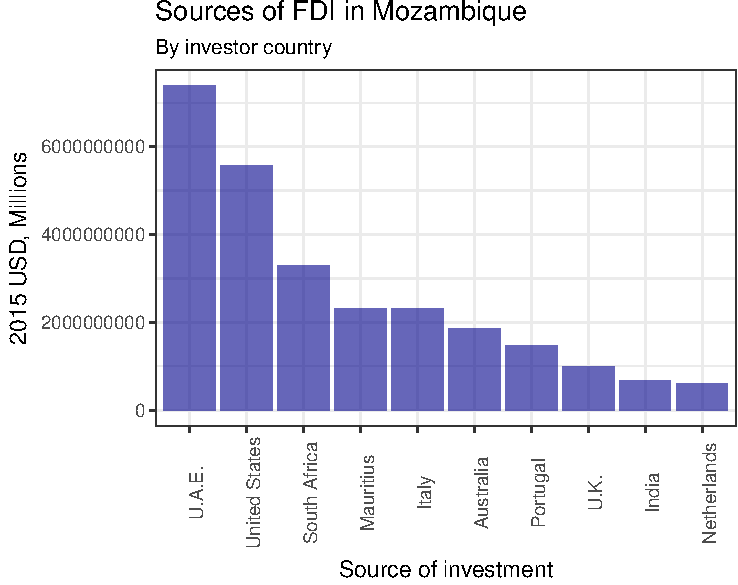
\includegraphics{figures/unnamed-chunk-7-1} \end{center}

What stands out is the presence of many ``non-Western'' countries in the
top 10. Though reliable data only go as far back as 2009, the landscape
of investment 20 years prior would have been both (a) far smaller and
(b) primarily composed of western countries, especially given that
Mozambique emerged so late from civil war (1994). Though as of 2015,
China did not figure in the top 10 FDI countries in Mozambique, its
upward trend is notable, with approximately 1.5 million USD invested in
2010 to nearly 100 million by 2015 (a 60-fold increase).

\subsubsection{Massive increase in FDI}\label{massive-increase-in-fdi}

Following independence (1974), Mozambique saw two decades of low and
unsteady foreign investment, largely due to the civil war (which did not
end until 1992). Thereafter, foreign investment began a steady increase
but leveled off by the late 1990s. However, the discovery of novel
sources of oil and gas set off a new spur of investments beginning in
2007, and continuing through last year. From 2010 to 2013, foreign
direct investment grew from 1.26 to 6.70 billion USD, a more than
five-fold increase (WB 2015).

In addition to the discovery of new resources, recent growth has also
been fueled by political and economic reforms which have made it easier
for foreigners to do business in Mozambique. Of particular note,
inflation remained relatively low (at least through 2014) (Bundesbank
2015).

\begin{center}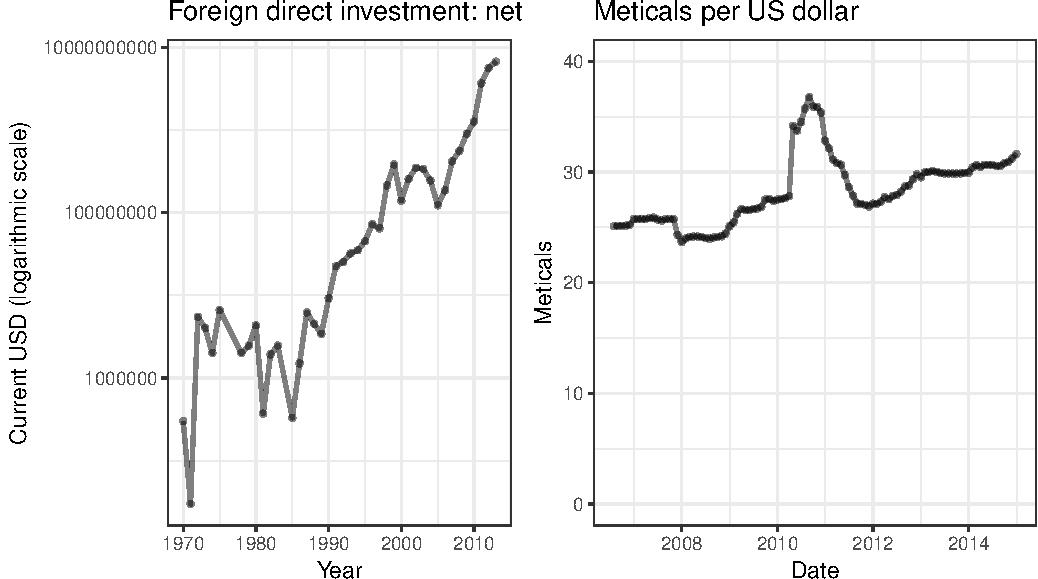
\includegraphics{figures/unnamed-chunk-10-1} \end{center}

The massive increases in FDI have also been facilitated by dramatic
decreases in the costs to import and export, as well as the costs of
starting a business and registering property (WB 2016).

\begin{center}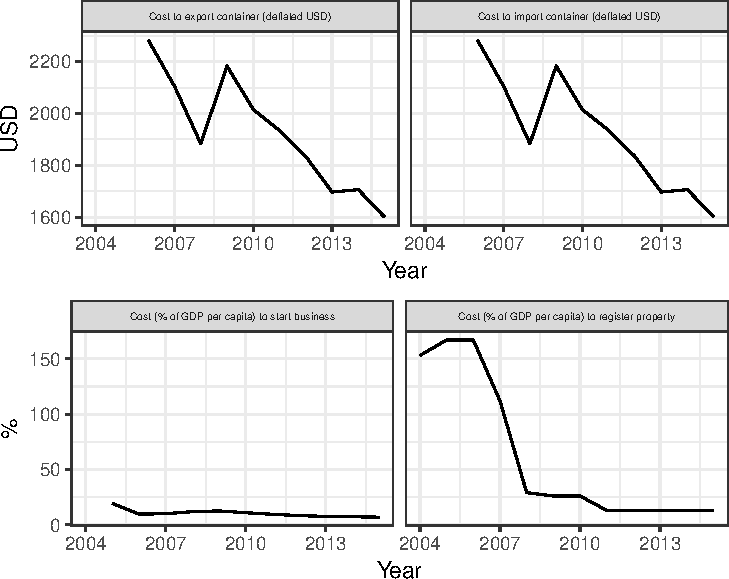
\includegraphics{figures/unnamed-chunk-11-1} \end{center}

\subsubsection{Breakdown by industry}\label{breakdown-by-industry}

Most of recent growth has come in the ``extractive'' industries, a term
encompassing a range of industry, but in the Mozambican context largely
applying to hydrocarbons and mining (INE 2015).

\begin{center}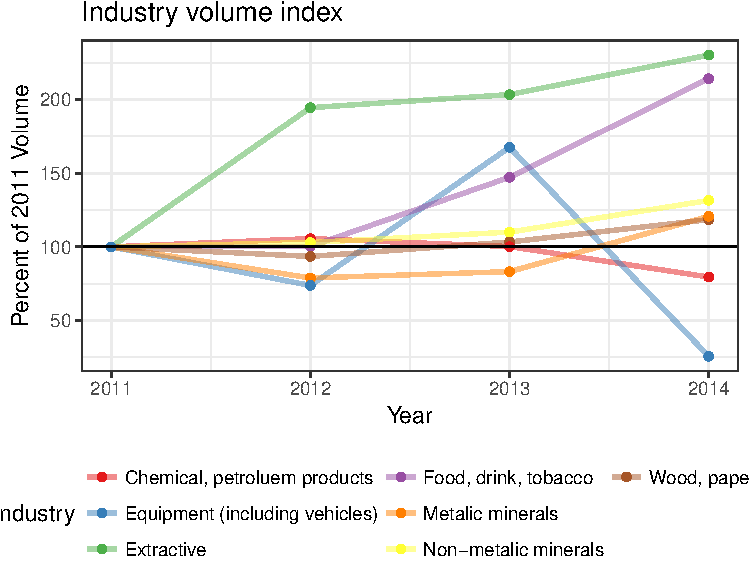
\includegraphics{figures/unnamed-chunk-12-1} \end{center}

The late 2015 economic slow-down in the developing world, particularly
the low price of oil, could have serious repercussions for FDI in
Mozambique. That said, the mining of metals and the service industries
both make up a larger share of Mozambique's economic output than the
extraction of hydrocarbons, which should somewhat buffer the Mozambican
economy from the negative effects of low oil prices.

\subsubsection{Breakdown by region}\label{breakdown-by-region}

Despite the concentration of private investment in regional projects,
growth has been similarly large in all provinces From 2000 to 2009, GDP
approximately doubled, with the greatest growth occurring in Inhambane
(119\% growth from 2000 to 2009), and the least robust grwoth in Nampula
(95\%) (Knoema 2015).

\begin{center}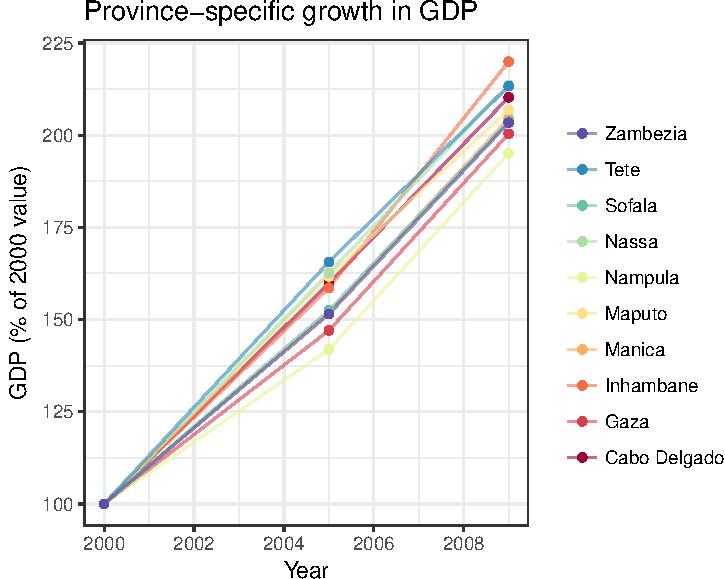
\includegraphics{figures/unnamed-chunk-13-1} \end{center}

The homogeneity in growth comes somewhat as a surprise, as it defies the
general developing world pattern in that growth in areas that already
had high GDP (Maputo and the coastal provinces) was as robust as growth
in areas with previously low GDP.

\begin{center}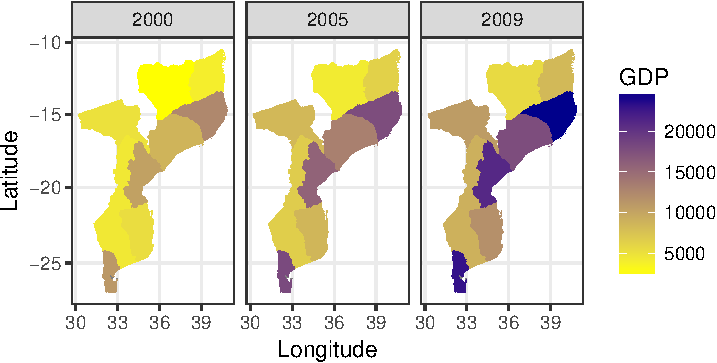
\includegraphics{figures/unnamed-chunk-14-1} \end{center}

FDI is associated with CSR. Whether under the guise of CSR or not, it is
noteworthy that the private sector currently does play a role in malaria
control activities. According to 2011 DHS data, greater than 7 in every
1,000 households had a private company carry out indoor residual
spraying (DHS 2011). And, in some clusters, the percent of houses
covered by private IRS was greater than 25\%.

Interestingly, though the UN data indicated that corporations don't
actively engage in malaria control as part of CSR, the geographic
distribution of households which had their homes sprayed by a private
entity are clustered in areas where foreign firms operate, particularly
in the south (around Maputo) in the East, where extractive industry
activity is highest.

\begin{center}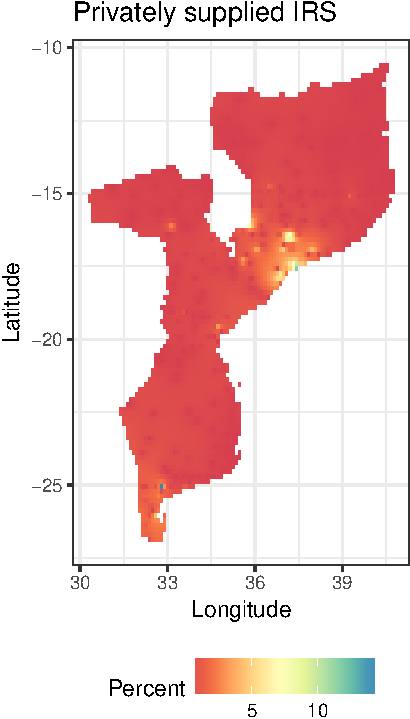
\includegraphics{figures/unnamed-chunk-16-1} \end{center}

\subsection{Systematic review}\label{systematic-review-1}

\subsubsection{Grey literature}\label{grey-literature-1}

\paragraph{Grey literature search
strategy}\label{grey-literature-search-strategy}

We devised 2 simple search queries, and use www.google.com and
www.bing.com to retrieve results. The queries were:

\begin{enumerate}
\def\labelenumi{\arabic{enumi}.}
\tightlist
\item
  \texttt{Mozambique\ foreign\ direct\ investment\ malaria}
\item
  \texttt{Mozambique\ corporate\ social\ responsibility\ malaria}
\end{enumerate}

\paragraph{Grey literature search
results}\label{grey-literature-search-results}

Google returned 266,000 results for the former query, and 240,000 for
the latter (506,000 in total); Bing returned 4,620 and 20,900,
respectively. We screened the top 50 results from both services (a total
of 100 items) for both queries For the former, of the 100 items
identified, 33 were identical in both search engines (yielding a total
of 67 unique items); in the latter, 39 were identical (yielding a total
of 61 unique items).

\begin{center}
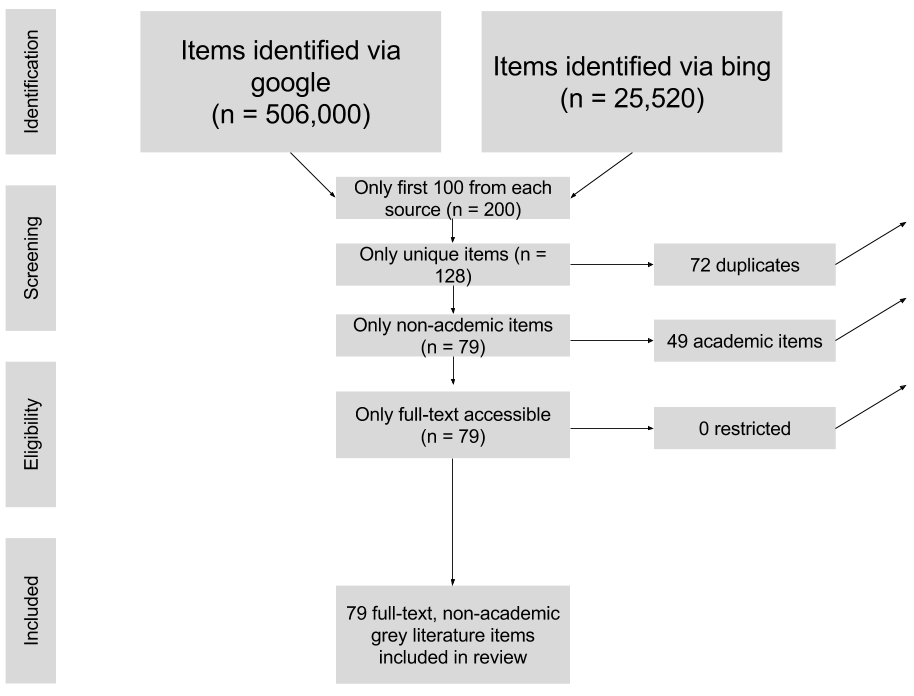
\includegraphics[width=400pt]{img/prisma_grey.png}
\end{center}

\paragraph{Grey literature synthesis}\label{grey-literature-synthesis}

Our grey literature review returned relatively little information which
was not readily available in those sources uncovered in the data review
and systematic review. Very few foreign companies operating in
Mozambique have any publicly available information regarding corporate
social responsibility activities.

Corporate social responsibility in Mozambique is new in nomenclature,
but activities which could be classified as CSR have existed for
decades. The number of firms actively engaging in CSR cannot be
ascertained (given the large and ever-changing number of small
businesses), but virtually all of the largest firms, both foreign and
domestic, have a CSR component.

Firms with CSR activities are often large and foreign. Among the largest
``key players'' in Mozambican CSR are Coca-Cola, British Petroleum and
Colgate-Palmolive. State conglomerates, such as Águas de Moçambique and
Electricidade de Moçambique, also participate in CSR activities (Compact
2007). Large communications firms, such as Vodacom and MCEL, and banks
(BIM and BCI) have a CSR component, but generally focus on culture,
environment and sport, avoiding activities which could either complement
or conflict with the health sector (Kaufmann and Simons-Kaufmann 2015).

Among major foreign companies, those operating in extraction -
particularly mining - appear to be the most involved with malaria. BHP
Billiton has been active in vector control support to the governments of
Mozambique, Swaziland, and South Africa, particularly in the early 2000s
(BHP 2014). Kropfmuhl AG and Vale, also mining companies, have carried
out CSR related to both community development and malaria control in
Northern Mozambique (Kaufmann and Simons-Kaufmann 2015).

Most CSR-funded activities are focused on education, community
development, women's rights and entrepreneurship. According to a UN
poll, none of the country's largest firms invest directly in
malaria-related CSR activities (Compact 2007). That said, a majority of
the firms interviewed by the UN indicated that one of the principal
reasons for investment in CSR is to complement government efforts. To
the extent that malaria accounts for more of the loss in
disability-adjusted life years in Mozambique than comparable countries
(IHME 2015), malaria control's lack of representation among core CSR
activities is a notable absence. One important exception is the
Nando's-lead Goodbye Malaria Trust, an umbrella organization which
inclues a development impact bond, the Goodbye Malaria initiative, and
partnerships with several other foreign firms operating in Mozambique.

\subsubsection{Academic literature}\label{academic-literature-1}

Our search is outlined in the below PRISMA-based diagram.

\begin{center}
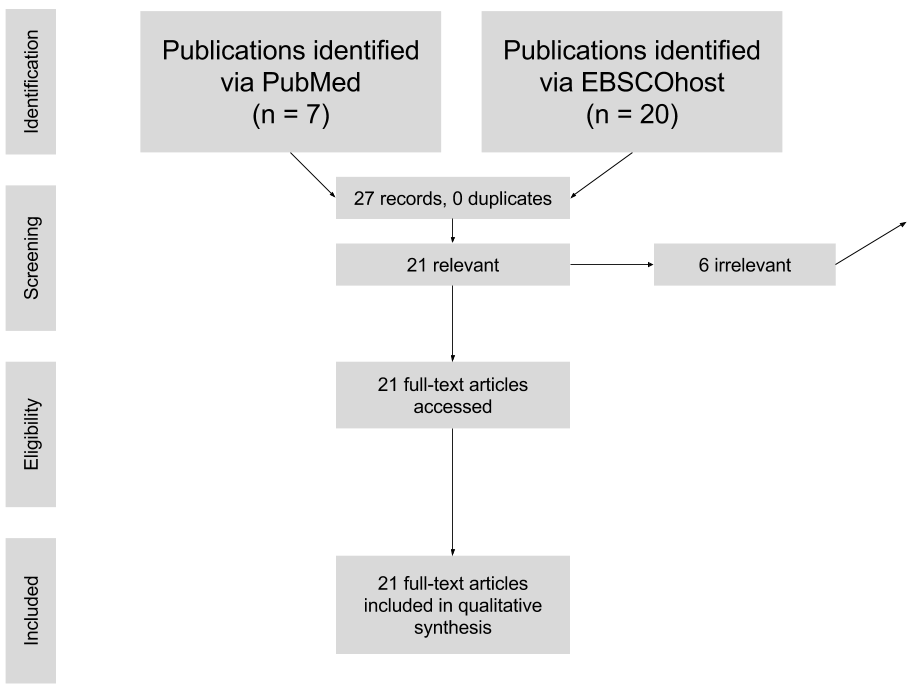
\includegraphics[width=400pt]{img/prisma.png}
\end{center}

The below table shows the results retrieved for the systematic review.
Full article information is in the bibliography

\begingroup\fontsize{6pt}{7pt}\selectfont

\begin{longtable}{lllll}
  \hline
Source & Year & Title & Type & Author \\ 
  \hline
EBSCOhost & 2009 & Public Governance, H... & FDI Malaria & Azemar, et al \\ 
  EBSCOhost & 2014 & A Critical Review of... & FDI MOZ & Mahembe, et al \\ 
  EBSCOhost & 2000 & Administrative barri... & FDI MOZ & Emery, et al \\ 
  EBSCOhost & 2012 & Attracting Foreign D... & FDI MOZ & Tembe, et al \\ 
  EBSCOhost & 2013 & Contemporary Process... & FDI MOZ & German, et al \\ 
  EBSCOhost & 2012 & Corruption and Multi... & FDI MOZ & Grande, et al \\ 
  EBSCOhost & 2014 & Determining the Natu... & FDI MOZ & Winkler, et al \\ 
  EBSCOhost & 1999 & Foreign Direct Inves... & FDI MOZ & Morisset, et al \\ 
  EBSCOhost & 2002 & Foreign Direct Inves... & FDI MOZ & Bassu, et al \\ 
  EBSCOhost & 2014 & Growth, Capital Accu... & FDI MOZ & Castel-Branco, et al \\ 
  EBSCOhost & 2007 & Linkage Between fore... & FDI MOZ & Wilson, et al \\ 
  EBSCOhost & 2012 & Mining FDI and Infra... & FDI MOZ & Robbins, et al \\ 
  EBSCOhost & 2013 & Potential and actual... & FDI MOZ & Winkler, et al \\ 
  EBSCOhost & 2004 & Regional integration... & FDI MOZ & Goldstein, et al \\ 
  EBSCOhost & 2014 & Sector Case Study: M... & FDI MOZ & Barnard, et al \\ 
  EBSCOhost & 2011 & Strategic Privatisat... & FDI MOZ & Buur, et al \\ 
  EBSCOhost & 2016 & The Economics and Po... & FDI MOZ & Hansen, et al \\ 
  EBSCOhost & 2002 & The Role of FDI in E... & FDI MOZ & Bjorvatn, et al \\ 
  EBSCOhost & 2010 & Uncovering Trends in... & FDI MOZ & Warren-Rodriguez, et al \\ 
  EBSCOhost & 2014 & Sector Case Study: A... & FDI MOZ & Barnard, et al \\ 
  Pubmed & 2004 & Community health out... & CSR & Singer, et al \\ 
  Pubmed & 2014 & Public-private partn... & CSR & Hutton, et al \\ 
  Pubmed & 2007 & Feasibility of water... & CSR MOZ & Tang, et al \\ 
  Pubmed & 2002 & The economic impact ... & FDI & Mills, et al \\ 
  Pubmed & 2004 & The economic burden ... & FDI & Russell, et al \\ 
  Pubmed & 2012 & The economic benefit... & FDI & Feachem, et al \\ 
  Pubmed & 2012 & Global health fundin... & FDI & D'Agostino, et al \\ 
  Pubmed & 2015 & Tracking Global Fund... & FDI & Huntington, et al \\ 
   \hline
\hline
\end{longtable}

\endgroup

The below chart shows our systematically retried publications by date.
What is most striking is how little academic attention has been given to
CSR, with none given to the intersection of CSR and malaria.

\begin{center}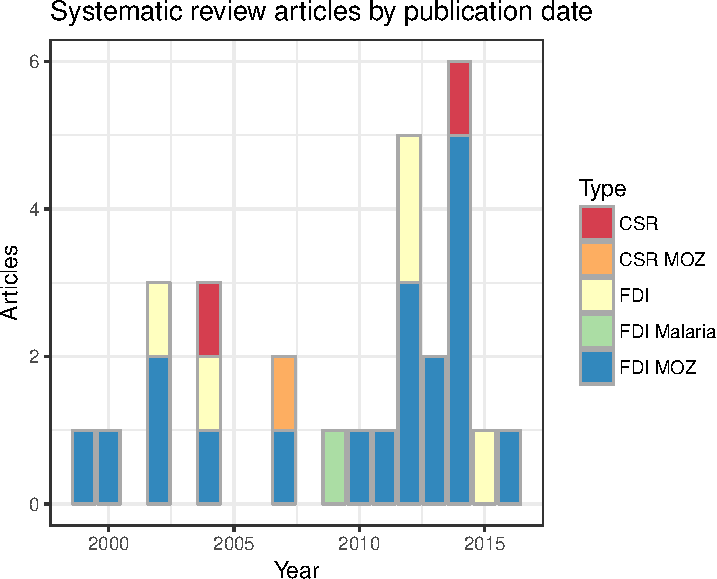
\includegraphics{figures/unnamed-chunk-19-1} \end{center}

\subsubsection{Qualitative synthesis of systematic review of academic
literature}\label{qualitative-synthesis-of-systematic-review-of-academic-literature}

The literature is largely clear on two points: (1) that economic growth
in Mozambique has been fueled in large part by foreign direct
investment, and (2) that economic growth has been accompanied by a rapid
decrease in malaria morbidity and mortality. There is no clear consensus
regarding the extent to which the former is a result of the latter, and
researchers disagree on how much of a role FDI has played in improving
the social and economic conditions of Mozambicans.

Mozambique has a unique social and economic system, which is
particularly attractive to foreign investment. The Mozambican economy is
``oriented to incentivize large-scale FDI projects'' (Robbins and
Perkins 2012). Land distribution, for example, despite being
igualitarian \emph{de juro} has been \emph{de facto} aimed at satisfying
the interests of large foreign firms (German, Schoneveld, and Mwangi
2013). In extractive industries, and particular the sugar industry, the
state has gone so far as to encourage unprofitable entreprise by
propping up an internal market so as to keep foreign inflows of cash
from drying out, a process described as a ``mediating bureaucracy''
(Buur, Tembe, and Baloi 2012). Another part of the attraction of FDI to
Mozambique is the extent to which the state and society, both formally
and informally, subsidize the cost of labor by allowing for below
subsistence wages.

In one view, the last two decades of economic growth are largely
irrelevant to the well-being of Mozambicans due to the ``porous and
extractive'' nature of FDI (Castel-Branco 2014). In other words, since
both investment and profit are largely external to the Mozambican
economy and society, ``positive spillovers'' into local firms are few
and far between (Winkler 2013).

CSR is one way of offsetting the trend, and its potential for mutually
beneficial effects is high, particularly when its resources target
malaria control. Per one analysis, malaria elimination in an endemic
country like Mozambique would lead to a 16\% increase in FDI (Azemar and
Desbordes 2009). The possibility of re-directing resource rents to
socially beneficial ends is acknolwedged by multiple authors (Robbins
and Perkins 2012, Castel-Branco (2014)).

However, the re-direction or resource rents to CSR is complicated. If
coerced (through higher taxes or fewer incentives to investment), the
recent decrease in FDI may be exacerbated. If voluntary, particularly in
the case of expenditures in medicine and health, the public's health
would be largely dependent on private whim, a recipe for
unsustainability at best and potential epidemiologic catastrophe at
worst.

In summary, Mozambique's high ratio of FDI to GDP and general allowance
of ``porous'' foreign investment represents an opportunity for scaling
up the private sector's engagement with public health, as a means to
offset the lack of social benefits that traditional FDI has entailed. A
coercive (tax-based) approach to scaling up this engagement may lead to
a withdrawl of FDI from the country. The alternative, an increase in
CSR, is a possible route for creating synergies, particular in the case
of malaria elimination.

\section{Discussion}\label{discussion}

The intensity of CSR activity seems to closely track FDI, but generally
avoids malaria control. The few malaria-related CSR projects in recent
years has come in large, ``mega-projects'' whose well-publicized malaria
abatement activities are profit-driven (Mouzin and al. 2011) or whose
primary aim is not profit-related (Han 2015). Though the former is often
portrayed as a ``win-win'' for business and public health, the latter
also offers tangible benefits for private industry, and should be
understood as operating under the same conditions and with the same
motivations. To the extent that most CSR activity has avoided the health
sector (including malaria) in favor of cultural, environmental,
education and more general ``development'' activities, it is reasonable
to assume that this may be due to the perceived costs of malaria
control, lack of perceived PR benefits, the government and NGO's
predominant role in the area, as well as the ``opt-in'' nature and
privacy/legal issues generally related to engaging in health-related
campaigns.

\subsection{Scaling up malaria control through CSR: opportunity and
risk}\label{scaling-up-malaria-control-through-csr-opportunity-and-risk}

\subsubsection{Opportunity}\label{opportunity}

The historical absence of malaria-related CSR represents an opportunity
for complementarity. In addition to improvements in public health, both
the private and public sectors stand to benefit economically from a
scaling up of malaria control driven by the private sector. By
increasing malaria control activities, as a share of total CSR
expenditures, public funds could be redirected towards other areas of
health. Likewise, if private CSR activities pivoted towards malaria
control rather more general philanthropical gestures, CSR would have a
more direct impact on wellbeing (with less temporal lag), thereby
fulfilling the public relations goals of the firms that invest in CSR.
Finally, for many industries, the firm itself is a potential direct
beneficiary, given that improvements in employee health and a reduction
in employee absenteeism can be directly correlated to productivity.

\subsubsection{Risk}\label{risk}

Scaling up CSR while also encouraging its redirection towards malaria
control is not without risks. The most notable downfall of this approach
is the potential for the inadvertent dependence on the private sector
for what is essentially a public good. Were CSR targeting malaria
control to reach significant levels (and the government were to enact a
correspoding redirection of funds towards the financing of other health
areas), then a situation would be created in which the public sector had
essentially divested from a public good. This would be unwise and
dangerous.

A secondary risk is that increased private sector involvement in malaria
control could cause a decrease in public sector \emph{competence} in the
prevention and treatment of malaria. This could have negative
consequences in the case of either a financial or economic crisis (in
which CSR activity would be curtailed) or an increase in malarial
activity. By the same token, CSR involvement in malaria control could
potentially portend, at least initially, less effective interventions.
Private firms' incentives, though aligned with the public's in terms of
malaria, are not identical, and pressures from shareholders and for
positive public perception might motivate malaria control strategies
which do not necessarily carry with them the most recent scientific
knowledge.

A third risk is a lack of coordination. Both in terms of logistical
activities as well as biological realities (drug and insecticide
resistance, etc.), coordination of malaria control activities is
absolutely essentially if Mozambique is going to make the transition to
eradication. The issue of coordination could be solved through an
activities and outcomes reporting/surveillance structure (necessarily
managed by the state), but compliance could be problematic.

A final risk is that of volatility. By centralizing malaria control
under the auspices of the government, public health authorities can
effectively distribute malaria control expenditures to where and when
they are most needed. If this control were only in the hands of private
firms, expenditure would likely transform into a function of
firm-specific profitability and shareholder incentives, as well as
market cycles. This could lead to a situation in which malaria control
activities are most prevalent in areas where the economy is strongest,
rather than areas where the need is greatest.

\section{Conclusion}\label{conclusion}

High FDI in Mozambique and growing interest in CSR both call for
increased reflection on the private sector's role in the delivery of
public goods. A refocusing of CSR expenditures into areas where the need
is greatest (specifically, malaria control) could lead to better health
and greater profits. This ``win-win'' for the public and private sectors
represents a rare opportunity, which deserves more discourse, research
and experimentation.

That said, the growing interest in CSR suggests both that (a) the need
for services exist and (b) that corporations (especially foreign firms)
have enough excess capital to finance these services. Both of these
factors suggest the need for a better-fitting taxation rate, and a more
efficient delivery of public services. That said, in the short-term,
increasing the efficiency and effectiveness of CSR activity through a
re-pivoting towards malaria control should remain a goal.

\begin{center}\rule{0.5\linewidth}{\linethickness}\end{center}

\section*{References}\label{references}
\addcontentsline{toc}{section}{References}

\hypertarget{refs}{}
\hypertarget{ref-Adams2016}{}
Adams, Jean, Frances C. Hillier-Brown, Helen J. Moore, Amelia A. Lake,
Vera Araujo-Soares, Martin White, and Carolyn Summerbell. 2016.
``Searching and Synthesising `Grey Literature' and `Grey Information' in
Public Health: Critical Reflections on Three Case Studies.''
\emph{Systematic Reviews} 5 (1). Springer Nature.
doi:\href{https://doi.org/10.1186/s13643-016-0337-y}{10.1186/s13643-016-0337-y}.

\hypertarget{ref-Alfaro_2006}{}
Alfaro, Laura, Areendam Chanda, Sebnem Kalemli-Ozcan, and Selin Sayek.
2006. ``How Does Foreign Direct Investment Promote Economic Growth?
Exploring the Effects of Financial Markets on Linkages,'' September.
National Bureau of Economic Research.
doi:\href{https://doi.org/10.3386/w12522}{10.3386/w12522}.

\hypertarget{ref-Almfraji_2014}{}
Almfraji, Mohammad Amin, and Mahmoud Khalid Almsafir. 2014. ``Foreign
Direct Investment and Economic Growth Literature Review from 1994 to
2012.'' \emph{Procedia - Social and Behavioral Sciences} 129 (May).
Elsevier BV: 206--13.
doi:\href{https://doi.org/10.1016/j.sbspro.2014.03.668}{10.1016/j.sbspro.2014.03.668}.

\hypertarget{ref-Asante_2011}{}
Asante, Kwaku P, Charles Zandoh, Dominic B Dery, Charles Brown, George
Adjei, Yaw Antwi-Dadzie, Martin Adjuik, et al. 2011. ``Malaria
Epidemiology in the Ahafo Area of Ghana.'' \emph{Malaria Journal} 10
(1). Springer Nature: 211.
doi:\href{https://doi.org/10.1186/1475-2875-10-211}{10.1186/1475-2875-10-211}.

\hypertarget{ref-Azemar2009}{}
Azemar, C., and R. Desbordes. 2009. ``Public Governance, Health and
Foreign Direct Investment in Sub-Saharan Africa.'' \emph{Journal of
African Economies} 18 (4). Oxford University Press (OUP): 667--709.
doi:\href{https://doi.org/10.1093/jae/ejn028}{10.1093/jae/ejn028}.

\hypertarget{ref-bhp}{}
BHP. 2014. ``BHP Billiton Case Study: Malaria.''
\url{https://www.bhp.com/-/media/bhp/documents/investors/reports/2004/norvatispresentation.pdf}.

\hypertarget{ref-NBERw17282}{}
Blonigen, Bruce, and Cheyney O'Fallon. 2011. ``Foreign Firms and Local
Communities.'' Working Paper 17282. Working Paper Series. National
Bureau of Economic Research.
doi:\href{https://doi.org/10.3386/w17282}{10.3386/w17282}.

\hypertarget{ref-Bloom2008}{}
Bloom, David, and David Canning. 2008. ``Population Health and Economic
Growth,'' 1--25.

\hypertarget{ref-World1999}{}
Brundtland, Gro Harlem. 1999. ``WHO on Health and Economic
Productivity'' 25 (2): 396--402.

\hypertarget{ref-deutsche}{}
Bundesbank. 2015. ``Exchange Rates for the Us Dollar in Mozambique / Usd
1 = Mzn.''
\url{https://www.quandl.com/data/BUNDESBANK/BBEX3_M_MZN_USD_CA_AC_A01}.

\hypertarget{ref-Burns_2017}{}
Burns, Darren K., Andrew P. Jones, Yevgeniy Goryakin, and Marc Suhrcke.
2017. ``Is Foreign Direct Investment Good for Health in Low and Middle
Income Countries? An Instrumental Variable Approach.'' \emph{Social
Science \& Medicine} 181 (May). Elsevier BV: 74--82.
doi:\href{https://doi.org/10.1016/j.socscimed.2017.03.054}{10.1016/j.socscimed.2017.03.054}.

\hypertarget{ref-Buur2012}{}
Buur, Lars, Carlota Mondlane Tembe, and Obede Baloi. 2012. ``The White
Gold: The Role of Government and State in Rehabilitating the Sugar
Industry in Mozambique.'' \emph{Journal of Development Studies} 48 (3).
Informa UK Limited: 349--62.
doi:\href{https://doi.org/10.1080/00220388.2011.635200}{10.1080/00220388.2011.635200}.

\hypertarget{ref-CastelBranco2014}{}
Castel-Branco, Carlos Nuno. 2014. ``Growth, Capital Accumulation and
Economic Porosity in Mozambique: Social Losses, Private Gains.''
\emph{Review of African Political Economy} 41 (sup1). Informa UK
Limited: S26--S48.
doi:\href{https://doi.org/10.1080/03056244.2014.976363}{10.1080/03056244.2014.976363}.

\hypertarget{ref-Compact2007}{}
Compact, U N Global. 2007. ``Corporate Social Responsibility: Country
Report Mozambique.''
\url{http://www.undp.org/content/dam/mozambique/docs/Poverty/UNDP}.

\hypertarget{ref-dhs}{}
DHS. 2011. ``USAID.''
\url{http://dhsprogram.com/what-we-do/survey/survey-display-362.cfm}.

\hypertarget{ref-Economist2017}{}
Economist. 2017. ``Mozambique's Default: Mozambique Fails to Pay Its
Debts.'' \emph{The Economist}, January. Economist.
\url{https://www.economist.com/news/middle-east-and-africa/21715030-mozambique-fails-pay-its-debts-mozambiques-default}.

\hypertarget{ref-Feenstra}{}
Feenstra, Robert, and Gordon Hanson. 1997. ``Foreign Direct Investment
and Relative Wages: Evidence from Mexico's Maquiladoras.'' \emph{Journal
of International Economics} 42 (3-4): 371--93.
\url{https://EconPapers.repec.org/RePEc:eee:inecon:v:42:y:1997:i:3-4:p:371-393}.

\hypertarget{ref-Friedman}{}
Friedman, Milton. 1970. ``The Social Responsibility of Business Is to
Increase Its Profits.'' \emph{Corporate Ethics and Corporate
Governance}. Springer Berlin Heidelberg, 173--78.
doi:\href{https://doi.org/10.1007/978-3-540-70818-6_14}{10.1007/978-3-540-70818-6\_14}.

\hypertarget{ref-gadm}{}
Gadm. 2009. ``GADM Database of Global Administrative Areas Version
1.0.''

\hypertarget{ref-German2013}{}
German, Laura, George Schoneveld, and Esther Mwangi. 2013.
``Contemporary Processes of Large-Scale Land Acquisition in Sub-Saharan
Africa: Legal Deficiency or Elite Capture of the Rule of Law?''
\emph{World Development} 48 (August). Elsevier BV: 1--18.
doi:\href{https://doi.org/10.1016/j.worlddev.2013.03.006}{10.1016/j.worlddev.2013.03.006}.

\hypertarget{ref-Godin2015}{}
Godin, Katelyn, Jackie Stapleton, Sharon I. Kirkpatrick, Rhona M.
Hanning, and Scott T. Leatherdale. 2015. ``Applying Systematic Review
Search Methods to the Grey Literature: A Case Study Examining Guidelines
for School-Based Breakfast Programs in Canada.'' \emph{Systematic
Reviews} 4 (1). Springer Nature.
doi:\href{https://doi.org/10.1186/s13643-015-0125-0}{10.1186/s13643-015-0125-0}.

\hypertarget{ref-Gonz_lez_2015}{}
González, Raquel, Orvalho J. Augusto, Khátia Munguambe, Charlotte
Pierrat, Elpidia N. Pedro, Charfudin Sacoor, Elisa De Lazzari, et al.
2015. ``HIV Incidence and Spatial Clustering in a Rural Area of Southern
Mozambique.'' Edited by Jean KEditor Carr. \emph{PLOS ONE} 10 (7).
Public Library of Science (PLoS): e0132053.
doi:\href{https://doi.org/10.1371/journal.pone.0132053}{10.1371/journal.pone.0132053}.

\hypertarget{ref-Han}{}
Han, Lily. 2015. ``Malaria in Mozambique: trialling payment by
results.''
\url{http://www.theguardian.com/global-development-professionals-network/2014/mar/31/malaria-control-payment-by-results}.

\hypertarget{ref-ihme}{}
IHME. 2015. ``GBD Prifle: Mozambique.''
\url{www.medbox.org/gbd-profile-mozambique/download.pdf}.

\hypertarget{ref-imf}{}
IMF. 2003. ``International Monetary Fund's Foreign Direct Investment
Trends and Statistics.''
\url{https://www.imf.org/external/np/sta/fdi/eng/2003/102803.htm}.

\hypertarget{ref-estatistica}{}
INE. 2015. ``Economic Statistics.'' \url{http://www.ine.gov.mz/}.

\hypertarget{ref-ine}{}
---------. 2017. ``Instituto Nacional de Estatistica.''
\url{http://www.ine.gov.mz/}.

\hypertarget{ref-Kaufmann_2015}{}
Kaufmann, Friedrich, and Claudia Simons-Kaufmann. 2015. ``Corporate
Social Responsibility in Mozambique.'' \emph{CSR, Sustainability, Ethics
\& Governance}, December. Springer International Publishing, 31--50.
doi:\href{https://doi.org/10.1007/978-3-319-26668-8_2}{10.1007/978-3-319-26668-8\_2}.

\hypertarget{ref-knoema}{}
Knoema. 2015. ``GDP of Mozambique by Region, Province and Country.''
\url{http://knoema.com/atlas/Mozambique/ranks/GDP-at-Constant-Prices}.

\hypertarget{ref-Moonasar_2016}{}
Moonasar, Devanand, Rajendra Maharaj, Simon Kunene, Baltazar Candrinho,
Francisco Saute, Nyasatu Ntshalintshali, and Natashia Morris. 2016.
``Towards Malaria Elimination in the Mosaswa (Mozambique, South Africa
and Swaziland) Region.'' \emph{Malaria Journal} 15 (1). Springer Nature.
doi:\href{https://doi.org/10.1186/s12936-016-1470-8}{10.1186/s12936-016-1470-8}.

\hypertarget{ref-Mouzin2011}{}
Mouzin, Eric, and Et al. 2011. ``Business Investing in Malaria Control:
Economic Returns and a Healthy Workforce for Africa.'' \emph{Progress \&
Impact Series}, no. 6.

\hypertarget{ref-Nonvignon_2016}{}
Nonvignon, Justice, Genevieve Cecilia Aryeetey, Keziah L. Malm, Samuel
Agyei Agyemang, Vivian N. A. Aubyn, Nana Yaw Peprah, Constance N.
Bart-Plange, and Moses Aikins. 2016. ``Economic Burden of Malaria on
Businesses in Ghana: A Case for Private Sector Investment in Malaria
Control.'' \emph{Malaria Journal} 15 (1). Springer Nature.
doi:\href{https://doi.org/10.1186/s12936-016-1506-0}{10.1186/s12936-016-1506-0}.

\hypertarget{ref-Ortega_2016}{}
Ortega, María Isabel, Samantha Sabo, Patricia Aranda Gallegos, Jill
Eileen Guernsey De Zapien, Antonio Zapien, Gloria Elena Portillo Abril,
and Cecilia Rosales. 2016. ``Agribusiness, Corporate Social
Responsibility, and Health of Agricultural Migrant Workers.''
\emph{Frontiers in Public Health} 4 (March). Frontiers Media SA.
doi:\href{https://doi.org/10.3389/fpubh.2016.00054}{10.3389/fpubh.2016.00054}.

\hypertarget{ref-Pazienza_2015}{}
Pazienza, Pasquale. 2015. ``The Relationship Between Co2 and Foreign
Direct Investment in the Agriculture and Fishing Sector of Oecd
Countries: Evidence and Policy Considerations.'' \emph{Intellectual
Economics} 9 (1). Elsevier BV: 55--66.
doi:\href{https://doi.org/10.1016/j.intele.2015.08.001}{10.1016/j.intele.2015.08.001}.

\hypertarget{ref-Pfeiffer_2017}{}
Pfeiffer, James, Sarah Gimbel, Baltazar Chilundo, Stephen Gloyd, Rachel
Chapman, and Kenneth Sherr. 2017. ``Austerity and the `Sector-Wide
Approach' to Health: The Mozambique Experience.'' \emph{Social Science
\& Medicine} 187 (August). Elsevier BV: 208--16.
doi:\href{https://doi.org/10.1016/j.socscimed.2017.05.008}{10.1016/j.socscimed.2017.05.008}.

\hypertarget{ref-Porter2002}{}
Porter, KE, and MR Kramer. 2002. ``The Competitive Advantage of
Corporate Philanthropy.'' \emph{Harvard Business Review}, no. 80.
Harvard University Press.
doi:\href{https://doi.org/10.1186/s12936-016-1506-0}{10.1186/s12936-016-1506-0}.

\hypertarget{ref-Robbins2012}{}
Robbins, Glen, and David Perkins. 2012. ``MINING FDI AND INFRASTRUCTURE
DEVELOPMENT ON AFRICAS EAST COAST: EXAMINING THE RECENT EXPERIENCE OF
TANZANIA AND MOZAMBIQUE.'' \emph{Journal of International Development}
24 (2). Wiley-Blackwell: 220--36.
doi:\href{https://doi.org/10.1002/jid.2817}{10.1002/jid.2817}.

\hypertarget{ref-Rogers}{}
Rogers, Lina. 2014. ``Natural resources boom sustaining growth in
Mozambique.''
\url{http://www.abo.net/oilportal/topic/view.do?contentId=2195109}.

\hypertarget{ref-Selaya_2012}{}
Selaya, Pablo, and Eva Rytter Sunesen. 2012. ``Does Foreign Aid Increase
Foreign Direct Investment?'' \emph{World Development} 40 (11). Elsevier
BV: 2155--76.
doi:\href{https://doi.org/10.1016/j.worlddev.2012.06.001}{10.1016/j.worlddev.2012.06.001}.

\hypertarget{ref-Shahbaz_2015}{}
Shahbaz, Muhammad, Samia Nasreen, Faisal Abbas, and Omri Anis. 2015.
``Does Foreign Direct Investment Impede Environmental Quality in High-,
Middle-, and Low-Income Countries?'' \emph{Energy Economics} 51
(September). Elsevier BV: 275--87.
doi:\href{https://doi.org/10.1016/j.eneco.2015.06.014}{10.1016/j.eneco.2015.06.014}.

\hypertarget{ref-Sheela_2017}{}
Sheela, A.M., A. Ghermandi, P. Vineetha, R.V. Sheeja, J. Justus, and K.
Ajayakrishna. 2017. ``Assessment of Relation of Land Use Characteristics
with Vector-Borne Diseases in Tropical Areas.'' \emph{Land Use Policy}
63 (April). Elsevier BV: 369--80.
doi:\href{https://doi.org/10.1016/j.landusepol.2017.01.047}{10.1016/j.landusepol.2017.01.047}.

\hypertarget{ref-Sutton2014}{}
Sutton, John. 2014. \emph{MAPA Empresarial de Moçambique}. International
Growth Centre.
\url{http://personal.lse.ac.uk/sutton/mozambique_portuguese_edn_updated_version_web.pdf}.

\hypertarget{ref-Unctad2012}{}
UNCTAD. 2012. \emph{Investment Policy Review: Mozambique}. United
Nations.

\hypertarget{ref-wbdata}{}
WB. 2015. ``Foreign Direct Investment, Net Inflows (Bop, Current
Us\$).'' \url{http://data.worldbank.org/indicator/BX.KLT.DINV.CD.WD}.

\hypertarget{ref-doingbusiness}{}
---------. 2016. \emph{Doing Business 2016: Measuring Regulatory Quality
and Efficiency}. World Bank.
\url{http://www.doingbusiness.org/~/media/GIAWB/Doing\%20Business/Documents/Annual-Reports/English/DB16-Chapters/DB16-Mini-Book.pdf}.

\hypertarget{ref-wbd}{}
---------. 2017. ``World Bank Open Data.''
\url{https://data.worldbank.org/}.

\hypertarget{ref-White2014}{}
White, Nicholas J, Sasithon Pukrittayakamee, Tran Tinh Hien, M Abul
Faiz, Olugbenga A Mokuolu, and Arjen M Dondorp. 2014. ``Malaria.''
\emph{The Lancet} 383 (9918). Elsevier BV: 723--35.
doi:\href{https://doi.org/10.1016/s0140-6736(13)60024-0}{10.1016/s0140-6736(13)60024-0}.

\hypertarget{ref-World2016}{}
WHO. 2016. ``World Malaria Report.''
\url{http://apps.who.int/iris/bitstream/10665/252038/1/9789241511711-eng.pdf?ua=1}.

\hypertarget{ref-Williams_2015}{}
Williams, Brian G., Eleanor Gouws, Pierre Somse, Mpho Mmelesi, Chibwe
Lwamba, Trouble Chikoko, Erika Fazito, et al. 2015. ``Epidemiological
Trends for Hiv in Southern Africa: Implications for Reaching the
Elimination Targets.'' \emph{Current HIV/AIDS Reports} 12 (2). Springer
Nature: 196--206.
doi:\href{https://doi.org/10.1007/s11904-015-0264-x}{10.1007/s11904-015-0264-x}.

\hypertarget{ref-Winkler}{}
Winkler, Deborah. 2013. ``Potential and Actual FDI Spillovers in Global
Value Chains.''

\hypertarget{ref-Zhu_2013}{}
Zhu, Yan, Li-Yun Sun, and Alicia S. M. Leung. 2013. ``Corporate Social
Responsibility, Firm Reputation, and Firm Performance: The Role of
Ethical Leadership.'' \emph{Asia Pacific Journal of Management} 31 (4).
Springer Nature: 925--47.
doi:\href{https://doi.org/10.1007/s10490-013-9369-1}{10.1007/s10490-013-9369-1}.


\end{document}
